%
% Tallinn University of Technology - bachelor, master thesis template for LaTeX
%
% Public Version 1.1
% 2019 Adjusted by Frank Korving for his Bachelor Thesis, with contributions from Sander Arnus
%
% Public version 1.0
% 2010 - 2013 Thijs Nugteren and Joos Buijs for Master Thesis
%
% THIS IS THE MAIN FILE (i.e. compile this file, compiling the others directly won't work)
%
\documentclass[12pt, a4paper]{report}

% all the other includes etc. are done in the thesis.sty file.
\usepackage{thesis}

%
% These commands need to be defined in order to produce a correct and personalized document
%
\newcommand{\doctitle}{Software for Protein Determination}
\newcommand{\eestidoctitle}{Tarkvara Valkude Määramiseks}

\newcommand{\docsubtitle}{Bachelor Thesis}
\newcommand{\eestidocsubtitle}{Bakalaureusetöö}

\newcommand{\firstauthor}{Jaak Kütt}
\newcommand{\firststudentcode}{200814IAIB}
\newcommand{\secondauthor}{Georg Margus}
\newcommand{\secondstudentcode}{193294IAIB}
\newcommand{\thirdauthor}{Lauri Kask}
\newcommand{\thirdstudentcode}{193685IAIB}

\newcommand{\university}{TALLINN UNIVERSITY OF TECHNOLOGY}
\newcommand{\eestiuniversity}{TALLINNA TEHNIKAÜLIKOOL}

\newcommand{\school}{School of Information Technologies}

\newcommand{\department}{Department of Software Science}
\newcommand{\eestidepartment}{Infotehnoloogia teaduskond}

\newcommand{\supervisor}{Priit Järv}
\newcommand{\supervisortitle}{PhD}
\newcommand{\cosupervisor}{}
\newcommand{\cosupervisortitle}{}
\newcommand{\keywords}{protein determination, gel analysis, background subtraction, pixel intensity analysis}
\newcommand{\version}{1.0 version}
\newcommand{\monthYear}{May 2022}
\newcommand{\Year}{2022}
\newcommand{\signatureDate}{May 30th, 2022}

\author{
    \firstauthor\\
    \and
    \secondauthor\\
    \and
    \thirdauthor
}

%
% PDF settings
%
\hypersetup
{
    pdfauthor={
        \firstauthor\\
        \and
        \secondauthor\\
        \and
        \thirdauthor
    },
    pdfsubject={\doctitle},
    pdfkeywords={\keywords}
}

\begin{document}
\pagenumbering{roman}
\begin{titlepage}
\headheight = 57pt
\footskip = 5pt
\headsep = 0pt

\centering
\textsc{\begin{Large}
\university\\
\end{Large} }
\school\\
\department\\

\vspace*{7 cm}

\begin{center}

\firstauthor \quad \firststudentcode\\
\secondauthor \quad \secondstudentcode\\
\thirdauthor \quad \thirdstudentcode\\

\begin{Large}
\textsc{\textbf{\doctitle}}\\
\end{Large}
\docsubtitle\\
\end{center}

\begin{flushright}
\textbf{Supervisor}\\ \supervisor\\\supervisortitle\\
\end{flushright}

\vfill

Tallinn \Year
\end{titlepage}

\begin{titlepage}
\headheight = 57pt
\footskip = 5pt
\headsep = 0pt

\centering
\textsc{\begin{Large}
\eestiuniversity\\
\end{Large} }
\eestidepartment\\

\vspace*{7 cm}

\begin{center}

\firstauthor \quad \firststudentcode\\
\secondauthor \quad \secondstudentcode\\
\thirdauthor \quad \thirdstudentcode\\

\begin{Large}
\textsc{\textbf{\eestidoctitle}}\\
\end{Large}
\eestidocsubtitle\\
\end{center}

\begin{flushright}
\textbf{Juhendaja}\\ \supervisor\\\supervisortitle\\
\end{flushright}

\vfill

Tallinn \Year
\end{titlepage}



\normalsize

\chapter*{\centerline{Author’s Declaration of Originality}}\label{chapter:declaration}
\hfill \\
We hereby certify that we are the sole authors of this thesis. All the used materials, references
to the literature and the work of others have been referred to. This thesis has not been
presented for examination anywhere else.

\vskip1in
\begin{flushleft}
\begin{tabular}{p{2.0cm}p{6.2cm}p{3.8cm}}
  Author: & \firstauthor, \secondauthor, \thirdauthor & ......................................\\
  && \hfill(signature)\\
  Date: & \signatureDate &\\
  \\
  \\

\end{tabular}
\end{flushleft}


\chapter*{\centerline{Annotatsioon}}\label{chapter:abstract-eesti}
% Overwrite local hyphenation formatting to avoid contradicting est language rules
{
  \hyphenpenalty=100000
  \emergencystretch=\maxdimen

Bakalaurusetöö raames loodi Tallinna Tehnikaülikooli Küberneetikaosakonna Süsteemibioloogia laborile töölauarakendus. Rakenduse eesmärk on senise geelianalüüsi tööprotsessi optimiseerimine, kiirendades teatud toiminguid mis nõudsid ebavajalikul määral korduvaid liigutusi ja täpsust.

Tarkvara ehitati Qt raamistikule. Rakendus loodi Pythonis, kasutades PySide6 mähisteeki.
Andmetalletuseks on valida SQLite ja PostgreSQLi andmebaaside vahel, ning piltide laadimiseks failisüsteemi või OMERO andmebaasi.

Tulemuseks on tarkvaralahendus, mis suudab geelipilte sisse laadida, pildilt alamosa valida ning seda pöörata, ning teostada taustaeemaldust. Pildile saab paigutada radu, mille põhjal koostatakse intensiivsusgraafe, mida saab vajadusepõhiselt piiritleda nõutud pindala kättesaamiseks. Tulemusena saadud andmeid saab talletada andmebaasi hilisemaks ülevaatluseks ja analüüsiks.

Alguses planeeriti valminud rakendus avaldada publikule avatud lähtekoodiga, aga lõpupoole selgus, et rakendus pole veel piisavalt valmis, nõudes lisaviimistlusi.

Projekti GitLabi salv on leitav aadressilt \url{https://gitlab.cs.ttu.ee/jakutt/iaib}.

Lõputöö on kirjutatud inglise keeles ning sisaldab teksti 30 leheküljel, 8 peatükki, 25 joonist, 9 tabelit.

}

\pagebreak

\chapter*{\centerline{Abstract}}\label{chapter:abstract}
As part of this thesis, a desktop application for Tallinn University of Technology's Cybernetics Institute's Systems Biology laboratory was made. The goal was to optimize the current protein analysis workflow, speeding up certain tasks and operations that required unnecessary repetition and precision.

The software was built on the Qt framework. It was written in Python, using the PySide6 wrapper library. It uses either SQLite or PostgreSQL for data storage and the filesystem or OMERO for images. 

The result is a software that can load gel images and crop, rotate, perform background subtraction on them. Lane regions can be defined on the image for intensity plot generation, which can be cut off at places to extract desired areas. Those results can be stored in a database for later review and analysis.

The software was planned to be released to the public as an open-source project. Towards the end of development, however, it was considered not to be ready yet, requiring more polish.

The project's GitLab repository can be found at \url{https://gitlab.cs.ttu.ee/jakutt/iaib}.

The thesis is in English and contains 30 pages of text, 8 chapters, 25 figures, 9 tables.

\pagebreak

\chapter*{\centerline{List of Abbreviations and Terms}}\label{chapter:terms}
\begin{longtable}{p{3cm}p{10cm}}
API & Application Programming Interface \\
COX4 & Cytochrome c oxidase subunit 4, mitochondrial \\
CRUD & Create, Read, Update, Delete \\
CSS & Cascading Style Sheets \\
CSV & Comma-separated values \\
DBMS & Database Management System \\
GPLv3 & GNU General Public License version 3 \\
GUI & Graphical User Interface \\
HTML & Hypertext Markup Language \\
ORM & Object-relational mapper \\
OS & Operating system \\
ROI & Region of Interest \\
SQL & Structured Query Language \\
SSL & Secure Sockets Layer \\
UI & User interface \\
UX & User experience
\end{longtable}
\addtocounter{table}{-1} 

\pagebreak

\phantomsection
% Sets maximum depth of Table Of Contents
\setcounter{tocdepth}{2}
\renewcommand{\contentsname}{Table of Contents}
\tableofcontents

\clearpage \phantomsection
\setcounter{figure}{0}
\addcontentsline{toc}{chapter}{\listfigurename}
\listoffigures

\clearpage \phantomsection
\addcontentsline{toc}{chapter}{\listtablename}
\listoftables

\chapter{Introduction}\label{chapter:introduction}
\onehalfspacing
\setcounter{page}{0}
%from here on, start the 'real' page numbering, from 1, with normal digits
\pagenumbering{arabic}
\section{About \ganga \label{introduction}}

\par
This section of the workbook is intended to provide introductory
information on \ganga for people who know little, or nothing,
about it.

\subsection{Outline of functionality\label{functionality}}

\subsection{Web site\label{website}}

\subsection{Mailing lists\label{mail}}

\subsection{License \label{license}}



\chapter{Project Description}\label{chapter:project-description}
The goal was to develop an application that could automate the analysis of gels based on their protein content. The application was supposed to overcome certain limitations of alternative solutions. The clients also imposed certain requirements for the used technology stack and the type of application.

\section{Problem Outline}
The primary issue with the current method are its inefficiencies: the tools used to perform image analysis and store the results have a lot of repetitive, manual steps and require precision and consistency to avoid losing significant chunks of progress. Table \ref{table:time-costs} outlines the current steps and the reported time taken to perform them for one experiment, keeping in mind that making a mistake requires previous steps to be redone. Since at least three experiments are done, the total time taken can exceed 7.5 hours per protein.

\begin{table}[h!]
\small
\begin{tabular}{|p{0.15\linewidth} | p{0.60\linewidth} | p{0.15\linewidth}|}
 \hline
 \textbf{Order} & \textbf{Action} &  \textbf{Time taken} \\
 \hline
1 & Signal analysis & 10 minutes \\ \hline
2 & Ponceau analysis (normalization) & 10 minutes \\ \hline
3 & Cytochrome c oxidase subunit 4, mitochondrial (COX4) analysis (normalization by another protein) & 10 minutes \\ \hline
4 & Upload data to database & 120 minutes \\ \hline
 &  & \textbf{150 minutes} \\ \hline
\end{tabular}
\caption{Time costs of gel analysis}\label{table:time-costs}
\end{table}

Ponceau, signal, and COX4 analyses were performed using ImageJ. Data upload was done through a web interface for textual data and OMERO for images. The main pain points were using ImageJ for the analysis steps due to quirks of the software and data insertion through the web interface for the database, which was slow primarily from having to pick out relevant values from ImageJ results and performing repetitive creation/insertion operations using the web interface. 

\section{Requirements Analysis}

The requirements for the project were gathered in three phases: 1) initial outline and domain knowledge transfer, 2) use case analysis, 3) user flow validation through visual design.

\subsection{Initial Outline}

Initial meetings with the clients introduced the general technical and non-technical requirements for the software. Two significant goals were set out for the project. Primarily, the software should improve the speed of analysis done at the Systems Biology lab. Secondarily it should be published as open-source software under the GNU General Public License version 3 (GPLv3) to increase adoption by the scientific community.

To that end the first major requirement was that the software should be a desktop application to ease distribution and minimize the overhead required for individual scientists or labs using it. Since the clients wanted to retain the ability to maintain the software tools that they use, it was recommended that the project would be based on the Qt framework\footnote{https://www.qt.io/product/framework} which they were familiar with. It was agreed that since the authors were not that familiar with C++ which is native to Qt, a Python middleware framework would be used.

The software was supposed to support individual analysis work and a shared setting - the latter was modeled after the need to integrate with the client's existing systems: 1) PostgreSQL database, 2) OMERO image repository\footnote{https://www.openmicroscopy.org/omero/}.

This divide helped to identify different interested parties from whose perspectives were used to derive the requirements for the project: 1) project lead at the Systems Biology lab, 2) scientist working at the lab, 3) scientist working outside of the lab.

The only existing alternative software found during this phase was ImageJ, which was subsequently tested, and its documentation was used as a means to help derive a common domain vocabulary with the client.

\subsection{Use Case Analysis}

Three main use cases were identified: 1) preparing for analysis, 2) analyzing gel images, and 3) reviewing prior analysis results. Since it was concluded that the scientist working with the software would want to switch between these activities freely, a single user role representing the scientist was enough to describe the use cases.

\subsubsection{Preparing for Analysis}

The user should be able to describe the general context around the analysis, implemented as data table views. This includes:
\begin{itemize}
    \item describing the physical gel object and the samples added to its lanes;
    \item describing which types of measurements were done on which gel images.
\end{itemize}

\subsubsection{Analyzing Gel Images}

This is the primary use case of the software - the results obtained here are used in further scientific research outside of the application. 

The user should be able to select and modify the gel image on which to perform the analysis. Modifications include: 1) crop and rotate the area of interest, 2) subtract image background, and 3) specify the visual false-color mapping for the image. The user should be able to indicate where on the image specific lanes are positioned and how they are shaped. The user should be able to indicate the areas on which the pixel intensity analysis is performed, what is considered the signal, and what the background is, compare, and annotate the analysis results.

\subsubsection{Reviewing Prior Analysis}

The user should be able to view all previously defined general data and image analysis results without the fear of accidentally modifying anything. It was agreed that a button to toggle between the \emph{viewing} and \emph{editing} modes should always be present on the toolbar, clearly indicating which mode is currently active. The user should not be able to perform any actions which may result in data being modified when not in the editing mode. To simplify the review process the user should be able to search for the previously analyzed gels and measurements.

\subsection{User Flow Validation}

A month after the start of the project a longer meeting with the clients was held to finalize the use case details. As a result a mock-up of the application user interface (UI) views was drawn and finalized over several iterations of feedback from the clients. The visual look and user experience (UX) elements described with it also became part of the requirements. The mock-up can be seen in Appendix 1.

As a result of working through a visual means, a previously missing case of the main analysis flow was discovered leading to substantial changes in the existing implementation. 

\begin{figure}[H]
    \centering
    \includegraphics[width=0.5\textwidth]{figures/flow-before.png}
    \includegraphics[width=0.5\textwidth]{figures/flow-after.png}
    \caption[\textit{Change in the order of associations between components}]%
    {\textit{Change in the order of associations between components}}
    {\small {Top: initial order; Bottom: final order}}
    \label{fig:flow-change}
\end{figure}

\subsection{Identified User Stories}

Together with the initially identified interested parties and the requirements found for the scientist role during use case analysis, a total of 39 requirements were identified and described as user stories in tables \ref{table:requirements-lead} - \ref{table:requirements-scientist} of Appendix 2. The stories were divided as:

\begin{itemize}
    \item three from the perspective of the Systems Biology lab project lead;
    \item three from the perspective of a scientist working at the Systems Biology lab;
    \item four from the perspective of a scientist not working at the Systems Biology lab;
    \item 24 from the perspective of a scientist.
\end{itemize}

\section{Existing Solutions}

The main alternatives to our application are ImageJ and Image Lab. Neither of them fully covers the client's needs. A comparative table based on the requirements specified in the previous section can be found in Table \ref{table:alternative-comparison-results} of Appendix 4.

\subsection{ImageJ}

The existing (partial) alternative to our solution is ImageJ which is an image processing and analysis software for scientific usage. It lacks certain functionalities that our application aims to provide. 
Firstly, it does not offer the possibility to undo any actions during analysis. Mistakes made at later stages of analysis mean starting the process over again. Several hours of wasted time are possible because of that limitation. Our application does allow the user to correct their errors without discarding the whole analysis.
Also, ImageJ does not allow selecting curved regions on images. That means it is not possible to correctly analyze gel lanes if they happen to be curved. One of the requirements was to implement this functionality in our application.
It is also not possible to save any data, only to export the results to comma-separated values (CSV) file. Therefore scientists have to start their work all over again every time they want to analyze a new gel.

\subsection{Image Lab}

Image Lab is a software meant for imaging and analyzing gels and blots. It supports most of the same features as ImageJ, most notably adding the possibility to analyze curved lanes.
However, its main drawback is that it is not possible to save data to resume the work later. Only data export is provided \cite{image-lab}.

\section{Project Management}

Development work was organized in one-week-long sprint cycles. Meetings with the clients and supervisor took place on Mondays and focused mostly on verifying the implementations, prioritization, and acquiring domain knowledge. Planning meetings with the developers took place on Fridays (and later on Sundays), where issues were detailed and development times estimated. For estimations the average hours suggested by all developers was used with the addition of buffer time which was modified based on the performance of prior sprints. During the final few sprints, less effort was placed on time estimations since it was clear there was no time where to split or postpone their delivery.

Summaries of the meetings, as well as various documentation can be found on the GitLab Wiki page\footnote{https://gitlab.cs.ttu.ee/jakutt/iaib/-/wikis/home}. Most of the meetings and communication took place over Microsoft Teams\footnote{https://www.microsoft.com/en-us/microsoft-teams/group-chat-software}.

Milestones, issues, and source code was managed as a project on the university GitLab\footnote{https://gitlab.cs.ttu.ee/jakutt/iaib}. Feature development was done on separate branches and required approval from a reviewer before merging to the main branch.


\chapter{Project Design}\label{chapter:project-design}
This chapter will cover the frameworks and libraries used in the project, architectural choices made and the theoretical background for the method used to acquire user feedback.

The software architectural diagram is provided here for a general overview.

% Plantuml export, which then is exported to png
\begin{figure}[ht]
    \centering
    \includegraphics[width=1\textwidth]{figures/arhitecture-diagram.png}
    \caption{\textit{Software design.}}
    \label{fig:app-arh-diag}
\end{figure}

\section{Frameworks and Libraries}

\subsubsection{PySide6}
PySide6 is the framework used to develop the application. It is the official module for the Qt for Python project. It offers all of the UI elements and functionality provided by the Qt framework to be used in Python development \cite{pyside6}.

As an alternative, the PyQt \footnote{https://www.riverbankcomputing.com/software/pyqt/} library was initially considered due to being around longer and having more usage examples available online. After short testing with both PySide6 and PyQt components, it was apparent that their application programming interfaces (APIs) were similar enough to be mostly interchangeable. PySide6 was preferred as the officially supported framework with the knowledge that a larger example base was still available.

\subsubsection{PyQtGraph}
PyQtGraph is a graphics and graphical user interface (GUI) library intended for use in mathematical, scientific, and engineering applications \cite{pyqtgraph}. It is used in the project for selecting and visualizing ROIs on the Gel images, plotting intensity data, and manipulating limits for intensity analysis. It was chosen because of its high compatibility with the Qt framework, as well as for its selection of available components.

\subsubsection{NumPy}
NumPy is the fundamental package for scientific computing in Python. It ... provides a multidimensional array object, various derived objects (such as masked arrays and matrices), and an assortment of routines for fast operations on arrays ... \cite{numpy}. In the project, it is mainly used for manipulating the matrices containing the image data.

\subsubsection{PostgreSQL}
PostgreSQL is one of the most widely used object-relational database management systems \cite{postgresql}. In the application, it can be configured by the user to store the application data.
Support for PostgreSQL integration was required by the client so they could integrate the analysis results with in-house software directly. Supporting alternative databases was a consideration
and to that end, effort was made to simplify that process.

\begin{table}[h!]

\small
\begin{tabular}{|p{0.30\linewidth} | p{0.60\linewidth}|}
 \hline
 \textbf{Step} &  \textbf{File location} \\
 \hline
Implement adapter interface & iocbio/gel/gui/dialogs/database\_connection\_settings/ database\_connection\_settings.py\\ \hline
Add adapter to form & iocbio/gel/gui/dialogs/database\_connection\_settings/ db\_selection\_form.py\\ \hline
Add driver as a dependency & setup.py\\ \hline
\end{tabular}
\caption{Steps to add alternative database support}
\end{table}

\subsubsection{SQLite}
SQLite is a file-based Structured Query Language (SQL) engine for storing application data. It is a convenient option for storage due to its stand-alone nature and minimal configuration (path to file). The user can choose this option when locally stored data is acceptable. \cite{sqlite}

\subsubsection{SQLAlchemy}
SQLAlchemy is the Python SQL toolkit and Object-relational mapper (ORM) that gives application developers the full power and flexibility of SQL. It provides a full suite of well known enterprise-level persistence patterns, designed for efficient and high-performing database access, adapted into a simple and Pythonic domain language \cite{sqlalchemy}. It was chosen for the project for its popularity, extensive documentation and as a way to abstract the database layer for working with both PostgreSQL and SQLite.

\subsubsection{OMERO}
OMERO provides a complete platform for managing images in a secure central repository. It provides access to the images through a desktop app (Windows, Mac or Linux), from the web or from 3rd party software  \cite{omero}. Providing integration for importing Gel images from OMERO was one of the main requirements for the project. Communication with the OMERO server is handled by the OMERO.py \footnote{https://github.com/ome/omero-py} client library. 

\subsubsection{Alembic}
Alembic is a lightweight database migration tool for usage with the SQLAlchemy Database Toolkit for Python \cite{alembic}. This tool was chosen because of its compatibility with SQLAlchemy and ease of setup.

\subsubsection{Dependency Injector}

Dependency Injector is a dependency injection framework for Python \cite{di-framework}. An alternative framework, python-inject\footnote{https://github.com/ivankorobkov/python-inject}, was considered, but Dependency Injector was found to be more widely used and has better documentation.

\section{Architectural Choices}

\subsection{Dependency Injection}
Dependency Injection is a pattern that separates service configuration from the use of services within an application. It can help make it easier to see what the dependencies are and simplify testing by allowing to replace the real service implementations with stubs or mocks \cite{fowler-injection}.

Python applications rarely make explicit use of the pattern as the interpreted and dynamic nature of the language makes it unnecessary \cite{di-in-python}.

However, as the project advanced and the number of components which depended on the same services grew, it became evident that using a dedicated framework for managing dependencies would help to reduce the growing complexity. Dependency Injector framework was chosen and subsequently all of the component configurations were moved into a single Container class. That Container is responsible for injecting the object instances, factories, as well as configuration parameters to the components using constructor injection.

\subsection{Events}
Qt has a concept known as signals and slots. Signals are emitted by certain actions, for example, by clicking a button. Slots are functions that listen for emitted signals and perform appropriate tasks  \cite{signals-slots}.

Project software consists of various isolated views and components that nevertheless need to communicate with each other to keep different parts of the application synchronized. 
In the application events are managed by EventRegistry class which contains the definitions of all used signals. Every component that needs to emit or consume events could do it only through the injected EventRegistry instance. The main goals of this approach were to decrease the coupling between components, keep all the events defined in one place, and avoid the possibility of widgets emitting events that no other component of the system was listening to. It also helped to avoid the situation in which multiple different signals are actually signaling the same event.

\subsection{Undo/redo}

The software user is expected to perform a series of graph manipulations with the mouse during the intensity analysis. To avoid errors from accidental motions, the undo/redo mechanism was implemented using the Command pattern.

„The Command pattern lets toolkit objects make requests of unspecified application objects by turning the request itself into an object. This object can be stored and passed around like other objects. Use the The Command's Execute operation can store state for reversing its effects in the command itself. The Command interface must have an added Unexecute operation that reverses the effects of a previous call to Execute. Executed commands are stored in a history list. Unlimited-level undo and redo is achieved by traversing this list backwards and forwards calling Unexecute and Execute, respectively” \cite{gof-command}.

Data modifications were executed through a single HistoryManager instance, which stored the command objects for the current user scope. History was cleared when the user changed scope (either by navigating or switching application into viewing mode) to avoid accidentally executing events which were not visible anymore. Keeping the history through deletion and creation of objects was achieved using soft-delete flags and only performing the actual deletion when the scope changed.

\subsection{Database}

The application uses one database table for keeping track of the software migration versions and eight tables for storing the data which the user either entered directly in a form field or created with graph manipulation tools. Although most of the database tables and used types were a result of the initial requirements analysis and directly reflected the needs of scientific data, some choices deserve closer attention.

Originally the \emph{gel\_image} table was supposed to store both the values of its \emph{original\_file} and \emph{omero\_id} in a single field \emph{file\_location} since the application itself doesn't have a use for that separation on the database level. The client requested to store the \emph{omero\_id} separately so they could use that in conjunction with their in-house software.

All of the tables which are directly affected by the user have a boolean \emph{is\_deleted} field to support the undo/redo functionality.

Since SQLite stores numbers as floating-point numbers \cite{sqlite-numbers}, some of the numerical field types were also converted to floats instead of decimals. The loss in accuracy was estimated not to be an issue by the client. Fields in question are: 1) \emph{gel\_lane.protein\_weight}, 2) \emph{gel\_image.rotation}, 3) \emph{measurement\_lane.value}.

Fields storing relative locations of graphical elements used internally by the software are serialized and stored as text types on the database - since their values don't hold any meaning outside of the application context, there would be no benefit from using more complex field types like JSON. These fields are: 1) \emph{gel\_image.region}, 2) \emph{gel\_image\_lane.region}, 3) \emph{gel\_image\_lane.zero\_line\_points}.

The schema of the database is shown in Figure \ref{fig:app-db-erd} of Appendix 6.

\section{Measuring User Confidence}

During the active development of the project, emphasis was put on continuously discussing and verifying the algorithmic correctness of the required features. When the project started to fall behind in scope, features supporting the main gel image analysis flow were prioritized and tested by the client. But a lot of the features described to improve user interface and enhance user experience were discarded. By the end of the project, the authors were left with a question: the application is functional - is it also usable?

Corno et al. (2015) reviewed existing literature on how the role of the user is considered during software design and evaluation. A concept they paid closer attention to was the level of confidence the user had while interacting with technology. They note that user confidence is influenced by a correct and reliable system behavior. “One aspect of reliability, often neglected, is guaranteeing the consistency between system operation and user expectations, so that users may build confidence over the correct behavior of the system and its reaction to their actions” \cite{Corno2015}.

Since the number of people able to test our application was expected to be low and limited only to the available Systems Biology lab workers, no existing study methods were considered. 

To gain a better understanding of how the application met both the testers' expectations and user experience a Google Forms questionnaire was created. First, they were asked to identify their role by indicating whether they planned to use the software only while working at the lab or not. Then they were asked to indicate how confident they felt that the features listed worked and met their expectations. A scale of one (\emph{Not at all confident}) to five (\emph{Very confident}) was offered to allow the users to express their opinions more dynamically. The list of features covered in the questionnaire was derived from the user stories previously described in tables \ref{table:requirements-lead} - \ref{table:requirements-scientist}. Questions covered only the features that were implemented at the time of user testing.


\chapter{Software Description}\label{chapter:software-description}
The project was implemented as a desktop Python application capable of running on Windows and Unix-like operating systems. 

The application uses a SQL database to store both the operational and user-created data. If the user does not specify connection parameters for an external database the application creates a SQLite database file in the current working directory.

The application creates a cache directory under operating system (OS) provided temporary path. On Unix/Linux systems this is the path specified in the TMPDIR environment variable or \emph{/tmp} if TMPDIR is not defined. On Windows this is usually the path specified in the TEMP or TMP environment variable \cite{qt-dir}. Two types of files are written there: images fetched from OMERO and the results of image processing steps.

Credentials necessary to authenticate with the databases are stored using the Python keyring library. Therefore, on Windows the credentials are stored to Credential Locker, on macOS to Keychain and on UNIX-like systems to KWallet \cite{keyring}.

\section{Prerequisites and Installation}

The minimum required Python version to use the application is Python 3.8. It is recommended to use the Python virtual environment for installing and running the application (in the following steps, the virtualenv module\footnote{https://pypi.org/project/virtualenv/} is used). Due to an underlying dependency and the specific OS version the application is being installed on, an OS-specific C++ compiler may be required.

On Linux/Unix and macOS systems, the environment can be set up by running the following commands in the application root directory using a Unix shell program like Bash:
\begin{verbatim}
python -m virtualenv .venv 
source .venv/bin/activate
\end{verbatim}
The application can then be installed by running the following command:
\begin{verbatim}
python -m pip install -r requirements.txt .
\end{verbatim}
If previous steps produced no errors, then application can be executed by running the following command:
\begin{verbatim}
.venv/bin/iocbio-gel
\end{verbatim}

Installing and running the application on Windows is similar to the case of Linux. Commands can be run in Powershell or a similar command-line application.
Setting up the application:
\begin{verbatim}
py -m virtualenv .venv
.venv\Scripts\activate
\end{verbatim}
Installing the application:
\begin{verbatim}
py -m pip install -r requirements.txt .
\end{verbatim}
Running the application:
\begin{verbatim}
.venv\Scripts\iocbio-gel
\end{verbatim}

\subsection{Application Startup}

During the initial startup, the user is shown a database configuration dialog where it’s possible to specify the database management system (DBMS) to be used and the parameters to connect to the database, as well as an image source configuration dialog, where the user can choose between local filesystem storage or specify connection parameters to an OMERO server. The application tries to connect with given parameters and shows an error message if a connection can not be established. The user can then add the correct parameters. If the user closes the dialog, then the application does not proceed and is closed.

After the database connection has been established SQLAlchemy checks the migration history. Any unapplied migration scripts located at \emph{iocbio/gel/db/alembic/versions/*.py} will be run to ensure that the database schema conforms to the requirements of the application.

When the application is configured to connect to an OMERO instance, then, during the startup process, fresh copies of images are fetched from OMERO and stored in the local cache folder.

\section{Application Layout}
Visually the application is divided into three components: mostly static toolbar on top, a narrow navigation menu with embedded gels list on the left, and the main content area. 

\subsection{Toolbar}
The horizontal toolbar at the top of the application provides the user with access to both context-dependent and globally relevant functionalities. “Undo” and “Redo” buttons allow the user to revert their previous action or reapply previously reverted actions. “Current mode: Editing” and “Current mode: Viewing” either enable or disable the user's ability to modify objects and data. The “Settings” button acts as a link to the settings view. “Add new Gel” or “Add new Measurement” buttons
are available depending on the view and provide a shortcut for creating new objects.

\subsection{Navigation}
Left side of the application contains a “Gels” button which opens up the gels list view, a list of individually named gel buttons which lead the user to gel detail view for the selected gel and a “Types” button at the bottom, which opens the measurement types view.

\subsection{Content Area}
The main area which displays the views listed below. On the application startup the gels list view is displayed by default.

\section{Application Views}

The application views can be grouped into three different categories:
\begin{itemize}
    \item data tables which provide general overview of previous work and allow to specify context for the analysis - gels list view, gel detail view, measurement types view;
    \item gel image and graph manipulation views for the analysis steps - raw, adjust, background, lanes and measurements;
    \item settings view for changing the application configurations.
\end{itemize}

\subsection{Gel List View}
A table view where the user can navigate by clicking on the “Gels” button on the left upper corner of the application. The following columns are presented for every gel: ID, name, transfer, comment. In addition, the counts of attached lanes and measurements are shown. The value of every field except for the ID can be changed if the editing mode is active. The gel list view can be seen in Figure \ref{fig:gel-list}.

\subsection{Gel Detail View}
To navigate into the gel detail view one must click on one of the buttons with gel names on the left menu below the “Gels” button. On the upper part of the view, the gel name and creation time are displayed.
The lanes table contains the ID, lane number, sample ID, protein amount in micrograms (μg), comment fields, and a checkbox field indicating if it is a reference lane that samples can be compared to.
All fields except the ID can be changed if the editing mode is turned on. Lanes can also be deleted in this mode.
The measurements table contains the data of all the measurements linked to the gel. The table shows the image, time, ID, type, comment, and identifiers of connected lanes. All the fields can be changed in editing mode. The gel detail view can be seen in Figure \ref{fig:gel-detail}.

\subsection{Measurement Types View}
The measurements type view is a table view where one can navigate by clicking the “Types” button in the lower-left corner, below the gel buttons. The table shows the ID, name, and comment of every measurement type. The value of each field can be changed and the type can be deleted in editing mode. An error box appears and deletion fails if the user tries to delete a measurement type that is connected to one or more measurements. The measurement types view can be seen in Figure \ref{fig:types-list}.

\subsection{Gel Image Raw View}

The gel image view contains different sub-views meant for processing and analyzing the gel image. The user can move between these views by clicking on corresponding tabs.
The raw image view shows the gel image without any processing done on it. Image can not be changed in this view.

\subsection{Gel Image Adjust View}

Adjust view allows the user to specify a region on the image that is used for analysis in subsequent steps. A rectangle appears when the image is clicked. The size, rotation, and position of this rectangle can be changed by dragging it from the handles. The region can be confirmed for analysis by clicking on the “Apply” button. Adjust view can be seen in Figure \ref{fig:gel-image-adjust}.
\begin{figure}[ht]
    \centering
    \includegraphics[width=.5\textwidth]{figures/image-adjust-roi.png}
    \caption{\textit{Cropping/rotation selection ROI.}}
    \label{fig:types-list}
\end{figure}

\subsection{Gel Image Background View}

The background subtraction view gives the user the option to apply the rolling ball background subtraction algorithm, specifying kernel type (“ball”, “ellipsoid”, or “none”), ball radius (two radiuses for ellipsoid), and whether the image is inverted before passing into the algorithm. When “none” is chosen, background subtraction will not be performed). Pressing “Apply” will execute the algorithm with the given parameters. Three images are shown: how it looked from the previous step, the extracted background from the algorithm, and the result, which is the difference of the input image and background (matrix subtraction). If the image was set to be inverted, the algorithm will use an inverted version of the image and the result will be subtracted from the inverted image, which will then be inverted again to restore the original colors. The image should be inverted if the source image has a dark background. The rolling ball implementation used is the one from the scikit-image library \cite{rolling-ball}. The gel image background view can be seen in Figure \ref{fig:gel-image-bg-sub}.

\subsection{Gel Image Lanes View}
The lanes view contains an image graph with the image processed in the three previous views. The “New lane” button allows the user to place a vertical variable-width lane inside the bounds of the image, which will span from top to bottom. Existing lanes can be moved along the horizontal axis, change widths, or be removed entirely. The number of placeable lanes is bounded by the number of lanes defined in the gel detail view. 
For each lane, there is a corresponding graph showing the pixel intensities along the lane, the y-axis being the pixel intensity and the x-axis the position of the horizontal chunk of pixels in the lane, starting from the top of the lane. The graph has a modifiable zero-line below the reading that can be dragged around by their points, which can be added to the line by clicking on it. The resulting area for the lane is determined by the difference between the readings integral and zero-line integral from zero to the height of the lane. The gel image lanes view can be seen in Figure \ref{fig:gel-image-lanes}.

\begin{figure}[H]
    \centering
    \begin{subfigure}{.5\textwidth}
        \centering
        \includegraphics[width=0.9\linewidth]{figures/gel-image-lane-plot.png}
        \caption{Gel image lanes view: image plot with \\
        lanes L1 and L2.}
        \label{fig:sub-gel-image-lane-plot}
    \end{subfigure}%
    \begin{subfigure}{.5\textwidth}
        \centering
        \includegraphics[width=0.9\linewidth]{figures/gel-image-lane-graph.png}
        \caption{Gel image lanes view: graph for lane L1 zero-line in blue.}
        \label{fig:sub-gel-image-lane-graph}
    \end{subfigure}
    \caption{Gel image graph and lanes plot}
    \label{fig:gel-image-lane-graph-plot}
\end{figure}

\subsection{Gel Image Measurements View}

The measurements view contains four components: a) lanes' graph, b) intensity plots, c) measurement lanes table, and d) measurements table. (Figure \ref{fig:gel-image-measurements})

a) Image graph with the lanes marked on the previews analysis step. Placed lanes can't be manipulated in this view anymore.
Clicking on a lane allows the user to add or remove it from the selected measurement.

b) An intensity plot is shown for every selected lane for the current measurement.
Each plot shows the vertically combined pixel intensity values for every pixel row along the lane.
Minimum and maximum integration limit lines can be adjusted to specify what area of the plot should count toward the area of interest.

\begin{figure}[ht]
    \centering
    \includegraphics[width=0.6\textwidth]{figures/limit-lines.png}
    \caption[\textit{Integration limit lines}]%
    {\textit{Integration limit lines}}
    {\small {Shown as vertical yellow lines}}
    \label{fig:integration-limit-lines}
\end{figure}

c) An optional comment can be added to the measured area per lane and indicated whether the measurement was successful or not.

d) Measurement type and comment can be added. Clicking on a measurement row will mark that measurement as selected and update the information on other components to match that change.

\subsection{Settings View}
The user can navigate to the settings view by clicking on the “Settings” button on the toolbar. It allows the user to change configured database settings and offers the same options as the initial database dialog. The “Image source” section allows the user to choose between local and OMERO options for storing images. The “Database connection” section lets users specify the same database connection options as in the database configuration dialog. The settings view can be seen in Figure \ref{fig:settings}.

\subsubsection{Database Configuration}
The database configuration section lets the user choose between SQLite and PostgreSQL for the DBMS from the dropdown menu, and according to the choice specific configuration parameters will appear. In the case of SQLite, there are no additional settings to be shown. For PostgreSQL, the user can specify database host, port, Secure Sockets Layer (SSL) mode, database name, user, and password. This section will be shown to the user as a dialog when the application is first started and no database is configured.

\subsubsection{Image Source Configuration}
The image source configuration section lets the user choose the source for the images to be analyzed. The user can choose between a folder on the local filesystem and an existing OMERO database. If the local filesystem is chosen, files will be fetched from a folder in the application’s directory. If OMERO is selected, the user can specify the hostname, port, username, and password for the connection. This section is shown to the user as a dialog when the application is started and the image source has not been configured.


\chapter{Validation}\label{chapter:validation}
To validate if the goals set out by the project were successful, we rely on both comparing the list of features initially described as requirements and the results of user feedback testing.

28 out of the 39 identified user stories were implemented during the project. 27 of those were included in the user feedback questionnaire - one was excluded since it was only a requirement specific to the project lead at the Systems Biology lab - “I want the software to be released under GPLv3 license”. The questionnaire was filled out by three of the lab workers.

Summary of user feedback after testing:
\begin{itemize}
    \item testers felt very confident that 16 features worked and met their expectations;
    \item all but one feature - “I can use the software on macOS computer” - got at the highest confidence rating from at least one tester;
    \item average rating on a scale of one to five was 4.65.
\end{itemize}

The full result of the feedback can be seen in Table \ref{table:test-results} of Appendix 5.

General feedback from the client was that the software can perform the main use cases regardless of the features which were not finished. It can be used to manage the process and perform intensity analysis on gel images. Thus the primary project goal set during the start of the project was achieved.


\chapter{Results}\label{chapter:results}
Despite not meeting all the requirements set out at the start of the project, the authors were able to prioritize features supporting the primary goal of creating software that would reduce the gel analysis process time for the Systems Biology lab. The application allows a scientist to prepare and manage the gel context for analyses, measure protein sample quantities on the gel images and review prior work. The authors gained new knowledge and skills about used technologies, the development process, and the domain of the project.

An overview of which of the requirements were implemented can be seen in tables \ref{table:requirements-lead} - \ref{table:requirements-scientist} of Appendix 2.

Seven features that were part of the requirements for the secondary goal of making the software publicly available as an open-source project were not implemented:
\begin{itemize}
    \item I want GitLab pipeline configured to build packaged executables;
    \item I want the software to look as agreed on the UI design document;
    \item I want to use the software in my own language;
    \item I want to export the results of my work as a CSV file;
    \item I want to curve the lanes individually;
    \item I want a user manual for the software;
    \item I want the implementation of analysis steps formally documented.
\end{itemize}

\section{Internationalization}
At the ending phases of development, clients communicated the requirement for application to support other languages besides English. That would have been necessary for users whose first language is not English. PySide has a package for the convenient implementation of internationalization \cite{pyside-intl}, and therefore authors believe that adding such functionality will not be a big issue in the future. It was currently left out of the scope mainly because it was communicated too late.

\section{CSV Export}
Exporting gel and measurement data to Excel would have been useful for performing additional analysis in third-party software. Since it was not a high priority requirement, it was left out of the project scope due to time constraints. It should not be an overly complicated feature to add in the future, as generating CSV files from relational data is a relatively standard task.

\section{Curved Lanes}
The most prominent feature that was not implemented was the ability to select curved lanes for analysis. According to the clients, the need for that feature would be rare and only required when the physical gel gets damaged or distorted, but in that circumstance, it would be valuable. They estimated that a loss of a gel would result in two days of work to prepare another gel and that only if the study material is still available. Unfortunately, it did not get implemented as it was also one of the most complicated features.

\section{Gel Filtering}
The possibility to filter the gel list by search queries would be useful if there are many gels added. This would have also improved the user experience to a large degree. It was decided to leave it unimplemented due to it not being critical for application functioning and having more important features to implement at the time.


\chapter{Comments and Discussion}\label{chapter:comments}
This section provides analysis of the development process and an overview of important elements in the technology stack, with commentary on specific aspects during development that involved significant decisions or affected flow of development.

\section{Domain Knowledge}
At the time of choosing this topic for the thesis, we had little knowledge about protein determination methods and processes, how/what applications are used to perform analysis, and why. As we started working on the project and having meetings with the project owners, we received some details on the current way of processing gel images and their shortcomings. However, our understanding of how some features should work or relate to the processes was partially faulty for some aspects, which required some rework down the line. This may have been mitigated with more detailed communication and development of clearer specifications, and by periodically releasing partial versions of the applications for the project owner to test specific aspects of workflows. More thorough research into the backgrounds of the algorithms and motivations behind the methods, stepping into the scientist's shoes, may have also helped for some implementations.

\section{Project Management}

Two main causes were identified that contributed to a significant enough time delay and eventually resulted in cutting some features out of the scope - communication and external time management.

Although the features initially planned for the start of the project were simplistic, the authors spent a lot of time familiarizing themselves with the framework, libraries, and exact requirements of the project, but they did not take enough time to agree on development practices and communicate their specific implementation details before developing those features. This resulted in an initial codebase where duplication was hard to spot and rectify because of three varying styles of implementation - most of which required refactoring later on. 

It was an open discussion on whether or not the authors should have tried to more specialize in developing different aspects of the application. This would have perhaps decreased the combined time that was spent on individually learning all the frameworks and libraries. It would have also forced a stricter initial structure for the software and exposed the need to improve communication between the authors. Unfortunately, due to circumstances, the authors were able to work on the project on differing days of the week, and the communication overhead felt more like a blocker. Additionally, the initial development effort was placed on creating the different application views, and so at the time it made sense to focus everyone on creating vertical slices of the software.

Secondly, external time constraints were not properly taken into account in project management during the second half of the project. The authors were too optimistic in estimating their capabilities or available time and realized fairly late that the project scope should be reprioritized.

The project management process failed to properly identify which of the external time sinks were recurring in their nature and which were one-time events. This made planning issues for upcoming sprints more difficult. A strategy to cope with this was adopted in form of splitting the issues even smaller so it would be possible to pick them up more readily in an ad-hoc manner. It helped a little but was not a sufficient solution. When a developer fell behind on their input, the situation was compounded by the additional need to familiarize themselves with changes done in the software in the meanwhile. As a remedy, perhaps implementing pair-programming sessions would have helped, but the need for this was not communicated clearly at the time.

\section{Curved Lanes}
One of the initial requirements for the application, curved lanes, was eventually found to be notably difficult to implement, and therefore not implemented within the current scope. There was one idea of how it may be done relatively easily, using the MultiRectROI widget. It was a ready-made widget that allowed chaining together multiple rectangular ROIs at variable angles and would've provided a single concatenated array of image data, much like a regular ROI for easy usage \cite{multi-rect-roi}. The issue with it was that the ROIs when connected at angles, overlapped with each other at one side and left a gap on the other, which wouldn't have been the desired result. Other ideas revolved around creating polygonal ROIs that joined edge-to-edge and could have curved edges or simply two curved lines (PyQtGraph offers methods to implement curved lines using the PlotCurveItem class \cite{plot-curve-item}) from which the region data would be calculated with a custom-made algorithm, staying perpendicular to the centerline. Both of those ideas would have needed to solve the issue of curving causing one side to have fewer pixels than the other, meaning each rectangular row of pixels had to expand into a circular arc from the shorter line to and along with the longer. We had little idea of how to properly/most efficiently implement this and feared it would eat up too much time, so in the face of time constraints, we decided to drop it.

\section{Qt}
Using the Qt framework for our application was considered a given since it was desired by the project owner and deemed standard for the problem domain and user base. Since we were unfamiliar with the framework and making standard desktop applications, the rate of feature development was affected. It was difficult to tell if opting for a more familiar web-based app paradigm would've decreased initial friction and allowed us to implement more features, as some of the libraries for image processing and plotting might've been hard to find mature and feature-equivalent versions for. Performance implications were also considered, as some image processing algorithms are slow even in the current implementation. Visuals of the application may have been significantly better though, as Hypertext Markup Language (HTML) / Cascading Style Sheets (CSS) pages are easier to customize.

\section{Python}
We had the option to either use C++ or Python with a wrapper library for Qt, and we chose the latter due to familiarity and perceived ease of development when compared to the former. While the application might've been more performant on C++, the extra layer of unfamiliarity with the language, its lack of memory management, and fewer batteries-included libraries with usable widgets like PyQtGraph and skimage would have most likely increased the learning curve and development time for the same set of features significantly. The overall performance of the application, even with the overhead of Python, is good, with one exception being the background subtraction algorithm, which is implemented differently from its ImageJ equivalent.

\section{Application Architecture}
During the later stages of development, the authors found out about Qt's Model-View\footnote{https://doc.qt.io/qt-6/model-view-programming.html} system, which may have benefited the project significantly. Having a separate model object to more conveniently map the database entities and allow for easy state sharing across view components may have made implementing and maintaining some aspects, like Create, Read, Update, Delete (CRUD) tables for measurements and lanes, easier.
The documentation for it wasn't very in-depth, however, so the question of how to properly encode more complex views like graphs and integrate with other libraries remained and may have been too much of an undertaking by that stage of development.

\section{Alternative Image Sources}
Not nearly enough was done to support alternative image sources, as it was the case for adding databases. There is an interface \emph{select\_image.py}\footnote{iocbio/gel/gui/dialogs/select\_image.py} for implementing the visual dialog component which is shown to the user when attempting to select or change an image. But, since fetching images from a local folder didn't require managing a connection, a common interface for such a client was not created. As such, the first steps for implementing a new image source would be to follow the implementation and usage of the \emph{omero\_client.py}\footnote{iocbio/gel/application/image\_source/omero\_client.py} class and separate image source specifics from the shared interface.


\chapter{Conclusion and Future Development}\label{chapter:conclusion-future-development}
The project met its primary goal - the created application aids biologists sufficiently to be usable in laboratories for managing analysis process metadata and measuring the quantities of the protein samples on the gel images. During the project, 28 out of the 39 identified user stories were implemented, and the overall feedback from the client and the testers was positive.

The requirements for the secondary goal of being able to publish the software as an open-source project were not met due to time constraints. Some development was done towards that goal, but not all of the features were implemented or were implemented in a limited way.

In addition to finishing the missed functionality, there are some features that the authors believe could enhance the utility of the application.

Certain processes like lane and ROI detection, zero-line placement, and background detection could at least to some extent be automated. Zero-line placement should be relatively straightforward to implement as it is only necessary to determine the minimum value of the data and draw the horizontal line accordingly.

Currently, background subtraction is slow, partly because of the image dimensions. A possible option to reduce the time to run the rolling ball algorithm would be to downscale the image, apply the algorithm to get the background matrix, and then upscale the image again, and then subtract that from the original. The process could also be optimized by performing the background subtraction on a separate thread and avoiding freezing the UI. This way, the user could also stop the process if necessary.


\pagebreak
\phantomsection
\addcontentsline{toc}{chapter}{Bibliography}
\printbibliography

\pagebreak
\phantomsection
\appendix
\renewcommand{\thechapter}{\arabic{chapter}}

\clearpage
\phantomsection
\addcontentsline{toc}{chapter}{Appendix 1 – UI Draft}
\chapter*{Appendix 1 – Application UI Draft}
Design draft as agreed with the client as part of the requirements.

\begin{figure}[ht]
    \centering
    \includegraphics[width=1\textwidth]{figures/app-ui/main.png}
    \caption{\textit{Application layout.}}
    \label{fig:main}
\end{figure}

\begin{figure}[ht]
    \centering
    \includegraphics[width=1\textwidth]{figures/app-ui/gels-list.png}
    \caption{\textit{Application gels list view.}}
    \label{fig:gels-list}
\end{figure}

\begin{figure}[ht]
    \centering
    \includegraphics[width=1\textwidth]{figures/app-ui/gel-single.png}
    \caption{\textit{Application gels single view.}}
    \label{fig:gels-single}
\end{figure}

\begin{figure}[ht]
    \centering
    \includegraphics[width=1\textwidth]{figures/app-ui/raw-image.png}
    \caption{\textit{Application raw image view.}}
    \label{fig:raw-image}
\end{figure}

\begin{figure}[ht]
    \centering
    \includegraphics[width=1\textwidth]{figures/app-ui/adjust-image.png}
    \caption{\textit{Application adjust image view.}}
    \label{fig:adjust-image}
\end{figure}

\begin{figure}[ht]
    \centering
    \includegraphics[width=1\textwidth]{figures/app-ui/gel-background.png}
    \caption{\textit{Application gel background view.}}
    \label{fig:gel-background}
\end{figure}

\begin{figure}[ht]
    \centering
    \includegraphics[width=1\textwidth]{figures/app-ui/gel-lanes.png}
    \caption{\textit{Application gel lanes view.}}
    \label{fig:gel-lanes}
\end{figure}

\begin{figure}[ht]
    \centering
    \includegraphics[width=1\textwidth]{figures/app-ui/gel-measurements.png}
    \caption{\textit{Application gel measurements view.}}
    \label{fig:gel-measurements}
\end{figure}


\clearpage
\phantomsection
\addcontentsline{toc}{chapter}{Appendix 2 – User Stories}
\chapter*{Appendix 2 – User Stories}\label{appendix:user-requirements}
Requirements described as user stories of the identified roles.

\begin{table}[h!]
\small
\begin{tabular}{|p{0.02\linewidth}|p{0.80\linewidth}|p{0.15\linewidth}|}
\hline
   & \textbf{As the Systems Biology lab project lead} & \textbf{Implemented} \\
\hline
1 & I want the software to be released under GPLv3 license. & Yes\\ \hline
2 & I want GitLab pipeline configured to build packaged executables. & No\\ \hline
3 & I want the software to look as agreed on the UI design document. & No\\ \hline
\end{tabular}
\caption{Requirements of the Systems Biology lab project lead}\label{table:requirements-lead}
\end{table}

\begin{table}[h!]
\small
\begin{tabular}{|p{0.02\linewidth}|p{0.80\linewidth}|p{0.15\linewidth}|}
\hline
   & \textbf{As a scientist working at the Systems Biology lab} & \textbf{Implemented} \\
\hline 
4 & I want to import images from the lab’s OMERO server. & Yes\\ \hline
5 & I want my data saved on the lab’s PostgreSQL server. & Yes\\ \hline
6 & I want the software to indicate when it has lost external connections and allow to retry or change connection parameters. & No\\ \hline
\end{tabular}
\caption{Requirements of scientist working at the Systems Biology lab}\label{table:requirements-scientist-iocbio}
\end{table}

\begin{table}[h!]
\small
\begin{tabular}{|p{0.02\linewidth}|p{0.80\linewidth}|p{0.15\linewidth}|}
\hline
   & \textbf{As a scientist not working at the Systems Biology lab} & \textbf{Implemented}   \\ 
\hline
7 & I want to import images from my local computer. & Yes\\ \hline
8 & I want my data to persist between work sessions locally. & Yes\\ \hline
9 & I want to export the results of my work as a CSV file. & No\\ \hline
10 & I want to use the software in my own language. & No\\ \hline
\end{tabular}
\caption{Requirements of scientist not working at the Systems Biology lab}\label{table:requirements-scientist-not-iocbio}
\end{table}

\begin{table}[h!]
\small
\begin{tabular}{|p{0.02\linewidth}|p{0.80\linewidth}|p{0.15\linewidth}|}
\hline
   & \textbf{As a scientist} & \textbf{Implemented} \\
\hline
11 & I want to add and modify measurement types. & Yes\\ \hline
12 & I want to add and modify gels. & Yes\\ \hline
13 & I want to add and modify the general information about the lanes on the gel. & Yes\\ \hline
14 & I want to add multiple images for gels. & Yes\\ \hline
15 & I want to view the raw image before analysis. & Yes\\ \hline
16 & I want to select a ROI on the image before analysis (rotate and crop). & Yes\\ \hline
17 & I want to specify if the background on the image is dark or light. & Yes\\ \hline
18 & I want to correct image background (subtraction by rolling ball method). & Yes\\ \hline
19 & I want to choose a false-color mapping for the image. & Yes\\ \hline
20 & I want to mark the lane positions and widths on the Gel image. & Yes\\ \hline
21 & I want to adjust lane widths individually. & Yes\\ \hline
22 & I want to rotate the lanes individually. & No\\ \hline
23 & I want to curve the lanes individually. & No\\ \hline
24 & I want to see pixel intensity plots for marked lanes. & Yes\\ \hline
25 & I want to specify a zero-line to separate background from signal on the intensity plots. & Yes\\ \hline
26 & I want to add and modify measurements connected to specific gel images. & Yes\\ \hline
27 & I want to choose which lanes a measurement includes. & Yes\\ \hline
28 & I want to specify the integration limits on the pixel intensity plots. & Yes\\ \hline
29 & I want the selected limits to be visible on their lanes. & No\\ \hline
30 & I want to see a comparison and annotate analyzed lanes for measurements. & Yes\\ \hline
31 & I want to search previously analyzed gels by name, ID, sample ID, lane ID and measurement ID. & No\\ \hline
32 & I want the option to undo an accidental modification. & Yes\\ \hline
33 & I want a way to disable all editing operations to avoid accidental modifications during a review. & Yes\\ \hline
34 & I want to change my image and data source parameters after initial setup. & Yes\\ \hline
35 & I want to use the software on macOS computer. & Yes\\ \hline
36 & I want to use the software on Windows computer. & Yes\\ \hline
37 & I want to use the software on Linux computer. & Yes\\ \hline
38 & I want a user manual for the software. & No\\ \hline
39 & I want the implementation of analysis steps formally documented. & No\\ \hline
\end{tabular}
\caption{Requirements of a scientist}\label{table:requirements-scientist}
\end{table}


\clearpage
\phantomsection
\addcontentsline{toc}{chapter}{Appendix 3 – Application Views}
\chapter*{Appendix 3 – Application Views}\label{chapter:appendix-application-views}
\begin{figure}[ht]
    \centering
    \includegraphics[width=1\textwidth]{figures/views/gel-list.png}
    \caption{\textit{Application gel list view.}}
    \label{fig:gel-list}
\end{figure}

\begin{figure}[ht]
    \centering
    \includegraphics[width=1\textwidth]{figures/views/gel-lanes-popup.png}
    \caption{\textit{Application gel lanes popup view.}}
    \label{fig:gel-lanes-popup}
\end{figure}

\begin{figure}[ht]
    \centering
    \includegraphics[width=1\textwidth]{figures/views/types-list.png}
    \caption{\textit{Application measurement types list view.}}
    \label{fig:types-list}
\end{figure}

\begin{figure}[ht]
    \centering
    \includegraphics[width=1\textwidth]{figures/views/gel-detail.png}
    \caption{\textit{Application gel detail view.}}
    \label{fig:gel-detail}
\end{figure}

\begin{figure}[ht]
    \centering
    \includegraphics[width=1\textwidth]{figures/views/image-selection-popup.png}
    \caption{\textit{Application image selection popup view (local folder).}}
    \label{fig:gel-image-selection-popup}
\end{figure}

\begin{figure}[ht]
    \centering
    \includegraphics[width=1\textwidth]{figures/views/gel-image-raw.png}
    \caption{\textit{Application image raw view.}}
    \label{fig:gel-image-raw}
\end{figure}

\begin{figure}[ht]
    \centering
    \includegraphics[width=1\textwidth]{figures/views/gel-image-adjust.png}
    \caption{\textit{Application image adjust view.}}
    \label{fig:gel-image-adjust}
\end{figure}

\begin{figure}[ht]
    \centering
    \includegraphics[width=1\textwidth]{figures/views/gel-image-bg-sub.png}
    \caption{\textit{Application image background subtraction view.}}
    \label{fig:gel-image-bg-sub}
\end{figure}

\begin{figure}[ht]
    \centering
    \includegraphics[width=1\textwidth]{figures/views/gel-image-lanes.png}
    \caption{\textit{Application image lanes view.}}
    \label{fig:gel-image-lanes}
\end{figure}

\begin{figure}[ht]
    \centering
    \includegraphics[width=1\textwidth]{figures/views/gel-image-measurements.png}
    \caption[\textit{Application image measurements view.}]%
    {\textit{Application image measurements view.}}
    {\small {a) lanes graph}, {b) intensity plots}} \\
    {\small {c) measurement lanes table}, {d) measurements table}}
    \label{fig:gel-image-measurements}
\end{figure}

\begin{figure}[ht]
    \centering
    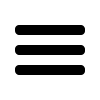
\includegraphics[width=1\textwidth]{figures/views/settings.png}
    \caption{\textit{Application settings view.}}
    \label{fig:settings}
\end{figure}


\clearpage
\phantomsection
\addcontentsline{toc}{chapter}{Appendix 4 – Requirements Comparison}
\chapter*{Appendix 4 – Requirements Comparison}
\small

\begin{longtable}[h!]{|p{0.02\linewidth} | p{0.7\linewidth} | p{0.05\linewidth}| p{0.05\linewidth}|}
\caption{Requirements satisfied by alternative applications}\label{table:alternative-comparison-results}\\
\hline
\rot{\textbf{Requirement No.}} & \rot{\textbf{Requirement}} & \rot{\textbf{ImageJ}} & \rot{\textbf{Image Lab}}\\
\hline
\endfirsthead
\multicolumn{4}{c}%
{\tablename\ \thetable\ -- \textit{Continued from previous page}} \\
\hline
\rot{\textbf{Requirement No.}} & \rot{\textbf{Requirement}} & \rot{\textbf{ImageJ}} & \rot{\textbf{Image Lab}}\\
\hline
\endhead
\multicolumn{4}{c}{\textit{Continues on next page}} \\
\endfoot
\hline
\endlastfoot
1 & I want the software to be released under GPLv3 license. & Yes & No\\ \hline
2 & I want GitLab pipeline configured to build packaged executables. & N/A & N/A\\ \hline
3 & I want the software to look as agreed on the UI design document. & N/A & N/A\\ \hline
4 & I want to import images from the lab’s OMERO server. & No & No\\ \hline
5 & I want my data saved on the lab’s PostgreSQL server. & No & No\\ \hline
6 & I want the software to indicate when it has lost external connections and allow to retry or change connection parameters. & N/A & N/A \\ \hline
7 & I want to import images from my local computer. & Yes & Yes\\ \hline
8 & I want my data to persist between work sessions locally. & No & No\\ \hline
9 & I want to export the results of my work as a CSV file. & Yes & Yes\\ \hline
10 & I want to use the software in my own language. & No & No\\ \hline
11 & I want to add and modify measurement types. & No & No\\ \hline
12 & I want to add and modify gels. & No & No\\ \hline
13 & I want to add and modify the general information about the lanes on the gel. & No & Yes\\ \hline
14 & I want to add multiple images for gels. & Yes & Yes\\ \hline
15 & I want to view the raw image before analysis. & Yes & Yes\\ \hline
16 & I want to select a ROI on the image before analysis (rotate and crop). & Yes & Yes\\ \hline
17 & I want to specify if the background on the image is dark or light. & Yes & Yes\\ \hline
18 & I want to correct image background (subtraction by rolling ball method). & Yes & Yes\\ \hline
19 & I want to choose a false-color mapping for the image. & Yes & Yes\\ \hline
20 & I want to mark the lane positions and widths on the gel image. & Yes & Yes\\ \hline
21 & I want to adjust lane widths individually. & No & Yes\\ \hline
22 & I want to rotate the lanes individually. & No & Yes\\ \hline
23 & I want to curve the lanes individually. & No & Yes\\ \hline
24 & I want to see pixel intensity plots for marked lanes. & Yes & Yes\\ \hline
25 & I want to specify a zero-line to separate background from signal on the intensity plots. & Yes & Yes\\ \hline
26 & I want to add and modify measurements connected to specific gel images. & N/A & N/A\\ \hline 
27 & I want to choose which lanes a measurement includes. & Yes & Yes\\ \hline
28 & I want to specify the integration limits on the pixel intensity plots. & Yes & Yes\\ \hline
29 & I want the selected limits to be visible on their lanes. & Yes & Yes\\ \hline
30 & I want to see a comparison and annotate analyzed lanes for measurements. & Yes & Yes\\ \hline
31 & I want to search previously analyzed gels by name, ID, sample ID, lane ID and measurement ID. & Yes & Yes\\ \hline
32 & I want the option to undo an accidental modification. & No & Yes\\ \hline
33 & I want a way to disable all editing operations to avoid accidental modifications during a review. & Yes & Yes\\ \hline
34 & I want to change my image and data source parameters after initial setup. & No & No\\ \hline
35 & I want to use the software on macOS computer. & Yes & Yes\\ \hline
36 & I want to use the software on Windows computer. & Yes & Yes\\ \hline
37 & I want to use the software on Linux computer. & Yes & No\\ \hline
38 & I want a user manual for the software. & Yes & Yes\\ \hline
39 & I want the implementation of analysis steps formally documented. & Yes & Yes\\
\end{longtable}


\clearpage
\phantomsection
\addcontentsline{toc}{chapter}{Appendix 5 – Questionnaire Results}
\chapter*{Appendix 5 – Questionnaire Results}
\begin{longtable}{|p{12cm}|p{1.5cm}|}
\caption{Questionnaire: user roles}\\
\hline
\textbf{Which of the following roles apply to you?} & \textbf{Answers}\\
\hline
\endfirsthead
\multicolumn{2}{c}%
{\tablename\ \thetable\ -- \textit{Continued from previous page}} \\
\hline
\textbf{Which of the following roles apply to you?} & \textbf{Answer} \\
\hline
\endhead
\hline \multicolumn{2}{c}{\textit{Continues on next page}} \\
\endfoot
\hline
\endlastfoot
I want to use the software only while working at the Systems Biology lab. & 3 \\ \hline
I am looking to use the software outside of the Systems Biology lab. & 3 \\
\end{longtable}


\begin{longtable}{|p{10cm}|p{0,5cm}|p{0,5cm}|p{0,5cm}|p{0,5cm}|p{0,5cm}|}
\caption{Questionnaire: user confidence}\label{table:test-results}\\
\hline
\textbf{Please answer how confident do you feel the following features work and meet your expectations on the scale of 1 (Not at all confident) to 5 (Very confident).} & \textbf{1} & \textbf{2} & \textbf{3} & \textbf{4} & \textbf{5}\\
\hline
\endfirsthead
\multicolumn{6}{c}%
{\tablename\ \thetable\ -- \textit{Continued from previous page}} \\
\hline
\textbf{Please answer how confident do you feel the following features work and meet your expectations on the scale of 1 (Not at all confident) to 5 (Very confident).} & \textbf{1} & \textbf{2} & \textbf{3} & \textbf{4} & \textbf{5} \\
\hline
\endhead
\hline \multicolumn{6}{c}{\textit{Continues on next page}} \\
\endfoot
\hline
\endlastfoot
I can import images from the lab’s OMERO server. & 0 & 0 & 0 & 0 & 3 \\ \hline
I can import images from my local computer. & 0 & 0 & 0 & 0 & 3 \\ \hline
My data is saved on the lab’s PostgreSQL server. & 0 & 0 & 0 & 0 & 3 \\ \hline
My data persist locally between work sessions. & 0 & 0 & 0 & 0 & 3 \\ \hline
I can add and modify measurement types. & 0 & 0 & 0 & 0 & 3 \\ \hline
I can add and modify gels. & 0 & 0 & 0 & 0 & 3 \\ \hline
I can add and modify the general information about the lanes on the gel. & 0 & 0 & 0 & 0 & 3 \\ \hline
I can add multiple images for gels. & 0 & 0 & 0 & 0 & 3 \\ \hline
I can view the raw image before analysis. & 0 & 0 & 0 & 0 & 3 \\ \hline
I can select and rotate a region on the image before analysis. & 0 & 0 & 0 & 0 & 3 \\ \hline
I can specify if the background on the image is dark or light. & 0 & 0 & 0 & 0 & 3 \\ \hline
I can correct image background. & 0 & 0 & 1 & 0 & 2 \\ \hline
I can choose a false-color mapping for the image. & 0 & 0 & 1 & 0 & 2 \\ \hline
I can mark the lane positions and widths on the gel image. & 0 & 0 & 0 & 1 & 2 \\ \hline
I can adjust lane widths individually. & 0 & 0 & 0 & 0 & 3 \\ \hline
I can see pixel intensity plots for marked lanes. & 0 & 0 & 0 & 1 & 2 \\ \hline
I can specify a zero-line to separate background from signal on the intensity plots. & 0 & 0 & 0 & 1 & 2 \\ \hline
I can add and modify measurements connected to specific gel images. & 0 & 0 & 0 & 0 & 3 \\ \hline
I can choose which lanes a measurement includes. & 0 & 0 & 1 & 0 & 2 \\ \hline
I can specify the integration limits on the pixel intensity plots. & 0 & 0 & 0 & 1 & 2 \\ \hline
I can see a comparison and annotate analyzed lanes for measurements. & 0 & 0 & 0 & 0 & 3 \\ \hline
I can undo an accidental modification. & 0 & 0 & 0 & 0 & 3 \\ \hline
I can disable all editing operations to avoid accidental modifications during a review. & 0 & 1 & 0 & 0 & 2 \\ \hline
I can change my image and data source parameters after initial setup. & 0 & 0 & 0 & 1 & 2 \\ \hline
I can use the software on macOS computer. & 1 & 0 & 2 & 0 & 0 \\ \hline
I can use the software on Windows computer. & 1 & 0 & 1 & 0 & 1 \\ \hline
I can use the software on Linux computer. & 0 & 0 & 0 & 0 & 3 \\
\end{longtable}


\clearpage
\phantomsection
\addcontentsline{toc}{chapter}{Appendix 6 – Database Schema}
\chapter*{Appendix 6 – Database Schema}
% Datagrip plantuml export, which then is exported to png
\begin{figure}[H]
    \centering
    \includegraphics[width=0.8\textwidth]{figures/app-db-erd.png}
    \caption{\textit{Application database entity relationship diagram.}}
    \label{fig:app-db-erd}
\end{figure}


\clearpage
\phantomsection
\small

\addcontentsline{toc}{chapter}{Appendix 7 – Non-exclusive licence for reproduction and publication of a graduation thesis}
\chapter*{Appendix 7 – Non-exclusive licence for reproduction and publication of a graduation thesis\footnote{The non-exclusive licence is not valid during the validity of access restriction indicated in the student's application for restriction on access to the graduation thesis that has been signed by the school's dean, except in case of the university's right to reproduce the thesis for preservation purposes only. If a graduation thesis is based on the joint creative activity of two or more persons and the co-author(s) has/have not granted, by the set deadline, the student defending his/her graduation thesis consent to reproduce and publish the graduation thesis in compliance with clauses 1.1 and 1.2 of the non-exclusive licence, the non-exclusive license shall not be valid for the period.}}

We Jaak Kütt, Georg Margus, Lauri Kask
\begin{enumerate}[label*=\arabic*.]
\item Grant Tallinn University of Technology free licence (non-exclusive licence) for our thesis "Software for Protein Determination", supervised by Priit Järv
  \begin{enumerate}[label*=\arabic*.]
    \item to be reproduced for the purposes of preservation and electronic publication of the graduation thesis, incl. to be entered in the digital collection of the library of Tallinn University of Technology until expiry of the term of copyright;
    \item to be published via the web of Tallinn University of Technology, incl. to be entered in the digital collection of the library of Tallinn University of Technology until expiry of the term of copyright.
  \end{enumerate}
\item We are aware that the authors also retains the rights specified in clause 1 of the non-exclusive licence.
\item We confirm that granting the non-exclusive licence does not infringe other persons' intellectual property rights, the rights arising from the Personal Data Protection Act or rights arising from other legislation.
\end{enumerate}

May 30th, 2022


\end{document}
